%*************************************************************
% Master Thesis                                             *
% Ing. Minerva Gabriela Vargas Gleason                       *
%  IAI - Institute of Artificial Intelligence                 *
% Universität Bremen                                         *
%                                                            *
% pdfLaTex                                                   *
% Editor: TeXnicCenter                                       *
%*************************************************************

\chapter{\textbf{Methodology}}

This chapter describes the general structure of the system developed in this work and all the elements that conform it. At the beginning, the perception system as well as the object's models are explained. A detailed description of the optimization-based motion controller can be found in section \ref{sec:motion_controller}, where several examples of basic controllers are presented. Afterwards, the controller developed for the robot is explained. In the end, the collision detection system is described.

\section{System description}
\label{sec:sys_description}

The system developed in this work, which has the objective of allowing the robot to identify and grab a specified object, comprises several parts:

\begin{itemize}
	\item \textbf{Object Database:} A database with a 3D model of the objects the robot will be able to grasp, as well as predefined grasping poses for each object.
	\item \textbf{Perception system:} In order to simplify the perception task, all objects are identified using markers. The position and orientation of the markers with respect to the reference frame of the objects is known.
	\item \textbf{Motion controller:} A constraint-based, optimization-based controller was developed. This controller allows the parametrization of the trajectory and automatically selects the best grasping pose according to the initial conditions.
	\item \textbf{Collision detection:} Since the motion controller is not able to detect collision objects in the environment, it is important to evaluate if the obtained trajectory would generate a collision
\end{itemize} 

A general description of the system's architecture is shown in figure \ref{fig:sys_arch}. The system uses ROS (section \ref{sec:ros}) to send and receive information from the robot and the user, each rectangle depicts a ROS node. All nodes communicate using ROS services, actions and messages.

\begin{figure}[H]
	\centering
	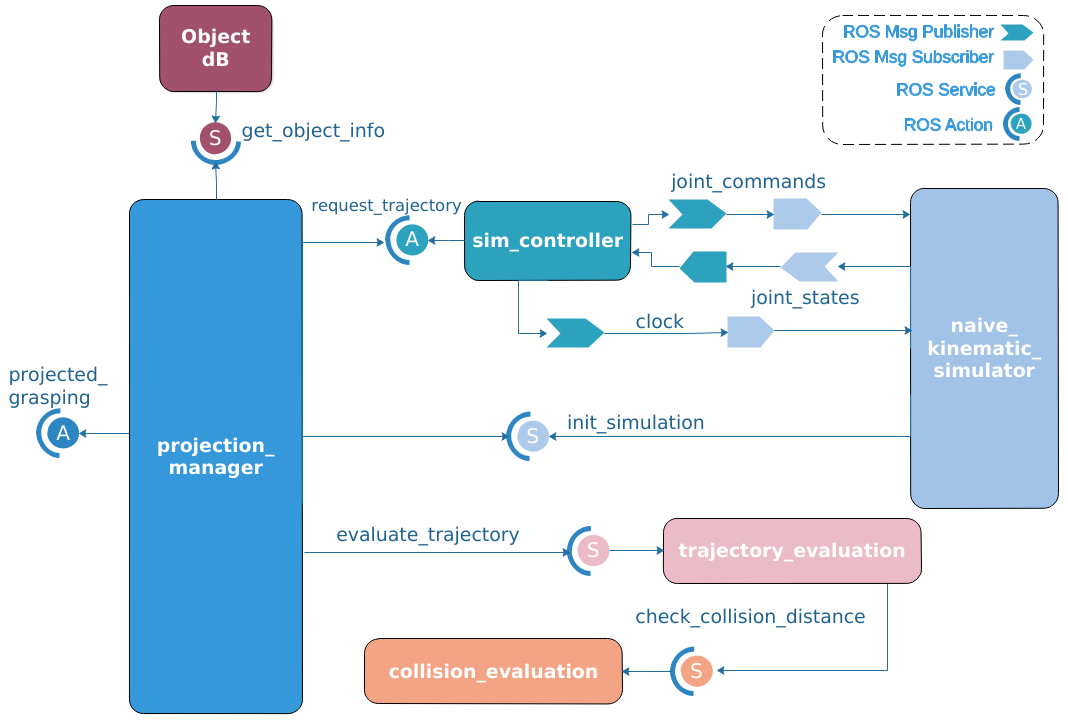
\includegraphics[width=1\linewidth, angle=0]{system/system-archit.png}
	\vspace{-10pt}
	\caption[System architecture] {System architecture: The perception system (\textit{Object\_dB}) sends location of found objects to the system manager (\textit{projection\_manager}), which requests a trajectory to the controller (\textit{sim\_controller}).}
	\vspace{-15pt}
	\label{fig:sys_arch}
\end{figure}

The \textit{Object dB} node is in charge of detecting objects and publishing its current location, as well as the defined grasping poses for each object. The object's information is read from a YAML file (section \ref{sec:db}). This node provides a service that publishes a list of found objects.

The component in charge of generating the trajectory is \textit{sim\_controller}, it receives the goal pose, calculates the required velocity for each joint, and sends it to the \textit{naive\_kinematic\_simulator}\footnote{https://github.com/code-iai/iai\_naive\_kinematics\_sim}, which simulates the robot's movements. It uses the controller described in section \ref{sec:motion_controller}.

The \textit{projection\_manager} node coordinates the whole system. It receives the request to grasp an object, asks the \textit{Object dB} if the object was detected and requests the generation of a trajectory to the motion controller. 

The \textit{projection\_manager} requests several trajectories to the \textit{sim\_controller} to have several options to choose from. It calculates the distance from both EEF to all the object's grasping poses. Based on the distance and the initial manipulability of each arm, selects the most suitable grasping pose (GP) and requests a trajectory to it, then discards this GP and selects the second best one and gets another trajectory. This process is repeated a couple of times to ensure that trajectories reaching different goals with both arms are obtained.

Then, \textit{projection\_manager} sends the trajectories to the \textit{trajectory\_evaluation} service (section \ref{sec:traj_eval}), which evaluates the trajectories, selects one and sends it back as result. 

The \textit{trajectory\_evaluation} service starts by sending each trajectory to the \textit{collision\_detection} service. If a collision is found, the trajectory is discarded. The remaining trajectories are scored based on length, smoothness, minimum distance to a collision object and the manipulability of the arm after reaching the goal. 

Once a trajectory is selected, the \textit{PI Controller} sends it to the robot and ensures that it follows the trajectory.

\section{Perception System}
\label{sec:perception}

The system requires previous knowledge about the objects the robot will interact with, it must be able to recognize the object and identify possible ways to grasp it. A 3D model of all objects was created, figure \ref{fig:model} shows an example of the models. These models are used for visualization in RVIZ. 
\begin{figure}[H]
	\centering
	\begin{subfigure}
		{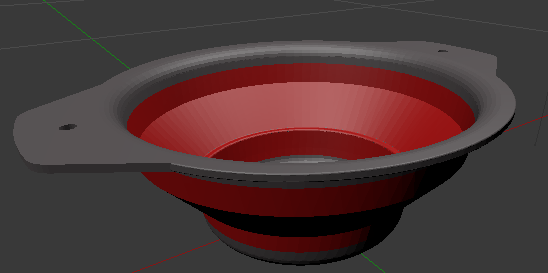
\includegraphics[width=0.34\linewidth]{bowl3.png}}
	\end{subfigure}
	\hspace{15pt}
	\begin{subfigure}
		{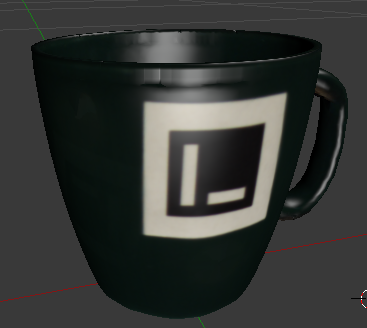
\includegraphics[width=0.2\linewidth]{cup3.png}}
	\end{subfigure}
	\vspace{-12pt}
	\caption[3D models]{DAE models of a bowl and a cup. On the cup, one of the markers used for perception can be seen.}
	\vspace{-10pt}
	\label{fig:model}
\end{figure}

In order to simplify the perception task, markers were added to all objects. The markers used are \textit{Chilitags}\footnote{http://chili.epfl.ch/software}, which can be integrated with ROS\footnote{https://github.com/chili-epfl/ros\_markers}. Once the tags or markers are detected by the camera, its position is published to a ROS topic. The \textit{Object dB} node matches the corresponding objects to the found markers and displays the models in RVIZ.

\subsection{Object Database}
\label{sec:db}
All the information about the objects is stored in a YAML file that works as database. The information is stored using the following structure:

\lstinputlisting[language=Python]{codes/db.yaml}

This structure is filled for every object the robot will grasp and added at the end of the YAML file.a

\subsection{Grasping Poses}

For humans, it is intuitive how an object can be grasped, but for a robot it is not a simple task. In this project, grasping poses (GP) are already defined for each object, so that the robot only has to choose which pose to use in every situation.
\begin{figure}[H]
	\centering
		{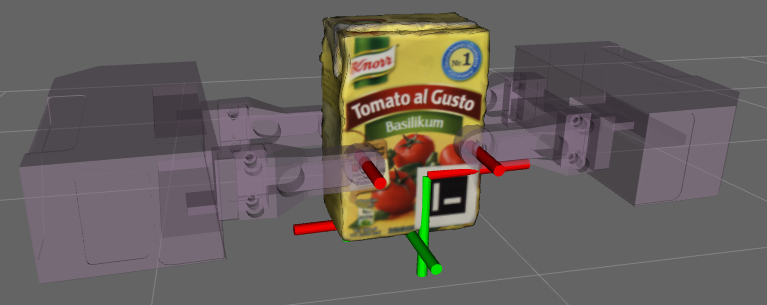
\includegraphics[width=0.5\linewidth]{knorr2.png}}
	\vspace{-12pt}
	\caption[Grasping poses]{3D model of a tomato sauce package with two grasping poses. The object and GP have reference frames.}
	\vspace{-10pt}
	\label{fig:knorr}
\end{figure}

Figure \ref{fig:knorr} shows an object with two predefined GPs. The perception system detects the position of the \textit{Chilitags} markers, searches the database for the corresponding object and GP and displays them in RVIZ, it also publishes a TF for both.


\section{Motion Controller}
\label{sec:motion_controller}

The motion control system used  to generate and control the movement of the robot is based on Giskard (section \ref{subsec:giskard}), an optimization-based controller. The controller developed in this work, as well as Giskard, uses \textit{qpOASES}\footnote{\url{https://projects.coin-or.org/qpOASES}}  to calculate a trajectory for each joint. A brief explanation of optimization-based controllers can be found in section \ref{sub:optimization}.

 As stated by \citet{qpoases},  qpOASES is an open-source optimization software that can solve quadratic programming (QP) problems of the form:
\begin{equation}
\underset{\vec{x}}{\min}\ c(\vec{x})\ =\  \underset{\vec{x}}{\min}\ \left( \frac{1}{2} \ \vec{x}\ ' \ \textbf{H} \ \vec{x} + \vec{x}\ ' \ \vec{g}(\omega_{0}) \right)
\label{eq:cost_in}
\end{equation}
Where $H \in \Re^{nV\times nV}$ is a symmetric and positive (semi-) definite Hessian matrix and $\vec{g} \in \Re^{nV}$ is a gradient vector that depends on the parameter $\omega_{0}$, with $nV$ being the length of the vector $\vec{x}$. The software tries to minimize the cost function $c(x)$. This minimization is subject to the following constraints:
$$\vec{lb}(\omega_{0})\ \leq\ \vec{x}\ \leq\ \vec{ub}(\omega_{0})$$
$$\vec{lbA}(\omega_{0})\ \leq\ \textbf{A}\vec{x}\ \leq\ \vec{ubA}(\omega_{0})$$
where $\vec{lb}$, $\vec{ub} \in \Re^{nV}$ are the lower and upper constraint bound vectors of $\vec{x}$, the matrix $\textbf{A} \in \Re^{nC\times nV}$ is the constrain matrix with the lower and upper constraint boundary vectors $\vec{lbA}$ and $\vec{ubA} \in \Re^{nV}$. Equality constraints can be achieved by setting equal upper and lower boundaries.
 
Several simple controllers were built and tested in order to understand the characteristics of the trajectories obtained using qpOASES. These controllers describe a two degree of freedom (DOF) linear manipulator. A state vector, $\vec{s}\ \in\ \Re^{nV}$, that describes the system is used as the variable the cost function minimizes:
\begin{equation}
 \vec{s} = [\dot{\ q_{0}} \ \ \dot{q_{1}} \ \ \epsilon ]^{T}
 \label{eq:state}
\end{equation}
where $\dot{q_{0}}$ is the velocity of the first joint, $\dot{q_{1}}$ the velocity of the second joint, and $\epsilon$ is a slack variable. Introducing this vector in the cost function (eq. \ref{eq:cost_in}) and setting the gradient $\vec{g}$ to zero:
\begin{equation}
\underset{\vec{s}}{\min}\ c(\vec{s})\ =\  \underset{\vec{s}}{\min}\ \left( \frac{1}{2} \ \vec{s}' \ \textbf{H} \ \vec{s} \right)
\label{eq:min_cost}
\end{equation}
with the minimization constraints given by:
\begin{equation}
\vec{lb}(t)\ \leq\ \vec{s}\ \leq\ \vec{ub}(t)
\label{eq:constrain}
\end{equation}
\begin{equation}
\vec{lbA}(t)\ \leq\ \textbf{A} \vec{s}\ \leq\ \vec{ubA}(t)
\label{eq:constrainA}
\end{equation}
We define different weights for each parameter of the state vector $\vec{s}$ by setting the $\textbf{H}$ matrix to:
$$
\textbf{H}\ =\ diag(\vec{\omega})
$$
with the weight vector $\vec{\omega} \in \Re^{nV}$. These weights allow us to prioritize the movement of one specific joint over the others, considering that the cost function for the 2 DOF controller from eq \ref{eq:min_cost} is given by:
\begin{equation}
c(\vec{s})\ =\ \frac{1}{2} \ \vec{s}' \ \textbf{H} \ \vec{s} =\ \frac{1}{2} \ (\ \dot{q_{0}}^{2}\omega_{1} + \dot{q_{1}}^{2}\omega_{2} + \epsilon^{2}\omega_{3})
\label{eq:cost}
\end{equation}

The software will try to minimize the cost of solving the problem by setting a higher value for the variables with a lower weight.

The result of this minimization problem is the velocity required by each joint to reach a goal position in a certain time. This can be set as an equality constraint:
\begin{equation}
error\ =\ q_{eef,\ des} - q_{eef}
\label{eq:init_error}
\end{equation}
\begin{equation}
error\ \ \leq\ \ \dot{\ q_{0}} + \dot{\ q_{1}} + \epsilon\ \ \leq\ \ error
\label{eq:goal}
\end{equation}
where $q_{eef,\ des}$ is the desired position of the end effector (EEF) and $q_{eef}$ the current position of the EEF. The position error can be used as a velocity goal if we suppose that we want to cover the distance error in one time unit. Velocity constraints are also established for each joint:
\begin{equation}
-\dot{q}_{0,max}\ \ \leq\ \ \dot{\ q_{0}}\ \leq\ \ \dot{q}_{0,max}
\end{equation}
\begin{equation}
-\dot{q}_{1,max}\ \ \leq\ \ \dot{\ q_{1}}\ \leq\ \ \dot{q}_{1,max}
\end{equation}
The software will try to find the velocity required by each joint to correct the position error in one time step. Since the joints have velocity limits, it might not be possible to set velocities that satisfy the constraint set by eq \ref{eq:goal} only using the joint velocities, that is why the slack variable $\epsilon$ was introduced, with the constraints: 
\begin{equation}
-\epsilon_{max}\ \ \leq\ \ \epsilon\ \leq\ \ \epsilon_{max}
\end{equation}
where $\epsilon_{max}\ \gg\ q_{0,max},\ q_{1,max}$. The weight of the slack value is higher than the ones of the joint velocities, so the software will try to give a higher value to the velocities than to the slack variable.

The joint limits also have to be taken into consideration:
\begin{equation}
(-q_{0,max} - q_{0})\ \ \leq\ \ \dot{\ q_{0}}\ \leq\ \ (q_{0,max} - q_{0})
\end{equation}
\begin{equation}
(-q_{1,max} - q_{1})\ \ \leq\ \ \dot{\ q_{1}}\ \leq\ \ (q_{1,max} - q_{1})
\end{equation}
These constraints will reduce the joint velocities when they are approaching the limits until they reach zero at joint limit. The obtained velocity is the velocity the joints would require to reach the goal position in one time instant. However, due to physical limitations, joints can not immediately reach maximum velocity in one time step, so acceleration limits have to be established:
\begin{equation}
-a_{0,max}\ \ \leq\ \ \dot{\ q_{0}}\ \leq\ \ a_{0,max}
\label{eq:accel0}
\end{equation}
\begin{equation}
-a_{1,max}\ \ \leq\ \ \dot{\ q_{1}}\ \leq\ \ a_{1,max}
\label{eq:accel1}
\end{equation}

 The maximum acceleration is calculated on every iteration using
 \begin{subequations}
 	\begin{align}
 		a_{n,max\_lim}\ \ =\ \ \frac{\dot{q}_{n,max} - a_{n,max}}{\dot{q}_{n,max}} + a_{n,max} \\
 		a_{n,min\_lim}\ \ =\ \ \frac{\dot{q}_{n,max} - a_{n,max}}{\dot{q}_{n,max}} - a_{n,max}
 	\end{align}
 	\label{eq:accel}
 \end{subequations}
where $n$ is the joint number and $a_{n,max}$ a constant acceleration limit. The acceleration constraint is calculated based on the current joint speed.

Combining equations \ref{eq:goal} to \ref{eq:accel1} to create the constraint bound vectors from equations \ref{eq:constrain} and \ref{eq:constrainA}, we obtain
\begin{equation}
\left( \begin{array}{c}
-\dot{q}_{0,max} \\
-\dot{q}_{1,max} \\
-\epsilon_{max} \\
\end{array}
\right)	\leq 
\left[ \begin{array}{cccc}
\omega_{1} & 0 & 0 \\
0 & \omega_{2} & 0 \\
0 & 0 & \omega_{3} \\
\end{array}
\right] *
\left( \begin{array}{c}
\dot{q}_{0} \\
\dot{q}_{1} \\
\epsilon \\
\end{array}
\right) 
\leq \left( \begin{array}{c}
\dot{q}_{0,max} \\
\dot{q}_{1,max} \\
\epsilon_{max} \\
\end{array}
\right)
\label{eq:state_constr}
\end{equation}
and \\
\begin{equation}
\left( \begin{array}{c}
error \\
-q_{0,max} - q_{0} \\
-q_{1,max} - q_{1} \\
a_{0,min\_lim} \\
a_{1,min\_lim} \\
\end{array}
\right)	\leq 
\left[ \begin{array}{cccc}
1 & 1 & 1 \\
1 & 0 & 0 \\
0 & 1 & 0 \\
1 & 0 & 0 \\
0 & 1 & 0 \\
\end{array}
\right] *
\left( \begin{array}{c}
\dot{q}_{0} \\
\dot{q}_{1} \\
\epsilon \\
\end{array}
\right) 
\leq \left( \begin{array}{c}
error \\
q_{0,max} - q_{0} \\
q_{1,max} - q_{1} \\
a_{0,max\_lim} \\
a_{1,max\_lim} \\
\end{array}
\right)
\label{eq:a_constr}
\end{equation}

The constrains set by these equations are the groundwork for the basic controllers explained in the following subsections. All these cases simulate a translational 2 DOF system, the goal is to place the EEF at a given position (goal position). The initial position of each joint is given, as well as a goal for the EEF. In these examples, the initial velocity and acceleration of the joints is assumed to be zero, but other initial conditions can be set.

\subsection{Simple 2 DOF controller}
A proportional gain, $p$, for the joints' goal is introduced in order to reduce the number of iterations the program requires to solve the problems. In other words, the proportional gain can be used to increase the joint velocities. This gain is added to equation \ref{eq:init_error}:
\begin{equation}
error\ =\ p\ *\ \left(q_{eef,des} - q_{eef}\right)
\end{equation}


Figures \ref{fig:basic_eef} and \ref{fig:basic} show the position and velocity of a 2 DOF manipulator, whose trajectory is calculated using equations \ref{eq:state_constr} and \ref{eq:a_constr} to obtain the joint velocity in each time step. Figure \ref{fig:basic_eef}  shows the EEF position (dashed), velocity and the goal position (dotted), while figure \ref{fig:basic} shows the position and velocity of the joints $q_{0}$ and $q_{1}$.

\begin{figure}[H]
	\centering
	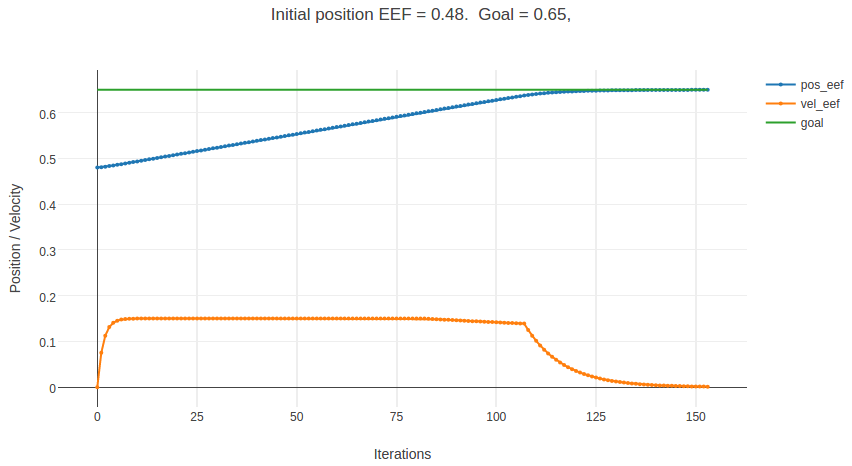
\includegraphics[width=0.7\linewidth, angle=0]{controllers/basic_eef.png}
	\vspace{-10pt}
	\caption[Basic 2 DOF controller: EEF trajectory.] {EEF trajectory. Initial acceleration is limited by constraints. Velocity decreases as EEF approaches the goal position.}
	\vspace{-15pt}
	\label{fig:basic_eef}
\end{figure}
\begin{figure}[H]
	\centering
	\begin{subfigure}[][Joint $q_{0}$]
		{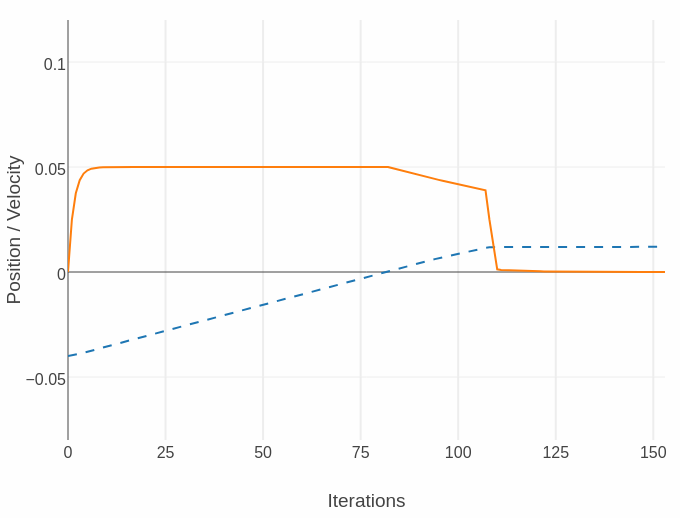
\includegraphics[width=0.49\linewidth]{controllers/basic_0.png}}
	\end{subfigure}
	\begin{subfigure}[][Joint $q_{1}$]
		{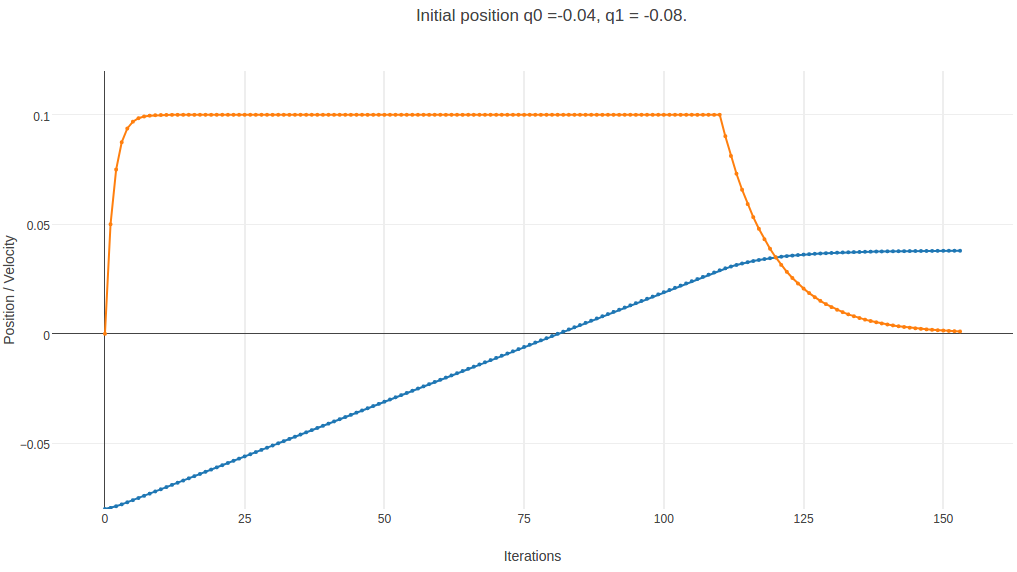
\includegraphics[width=0.49\linewidth]{controllers/basic_1.png}}
	\end{subfigure}
	\vspace{-12pt}
	\caption[Basic 2 DOF controller: Joints trajectories]{Joints trajectories (dashed). Each joint has different velocity (continuous line) and acceleration constraints.}
	\vspace{-10pt}
	\label{fig:basic}
\end{figure}
It can be seen that the velocity decreases once the EEF is approaching the desired position, also the joints do not reach the maximum velocity in the first time step. This is due to the acceleration constraint given by equation \ref{eq:accel}.

\subsection{Joints goal and EEF goal}
This controller allows to specify a goal position for one of the joints as well as for the EEF. Figures \ref{fig:joint_eef} and \ref{fig:joint_0} show the behavior of the EEF and both joints while reaching the specified goals. Each joint has different velocity and acceleration constraints.

In this controller, the weight vector is defined as $\vec{\omega} = [ \omega_{1},\ \omega_{2},\ \omega_{3},\ \omega_{4} ]$. Where $\omega_{1}$ and $\omega_{2}$ are the joint weights, $\omega_{3}$ is the weight of the slack factor and $\omega_{4}$ is the weight of the joint goal. Equation \ref{eq:a_constr} is rewritten as

$$
\left( \begin{array}{c}
error \\
-q_{0,max} - q_{0} \\
-q_{1,max} - q_{1} \\
a_{0,min\_lim} \\
a_{1,min\_lim} \\
joint\_error
\end{array}
\right)	\leq 
\left[ \begin{array}{cccc}
1 & 1 & 1 & 0 \\
1 & 0 & 0 & 0 \\
0 & 1 & 0 & 0 \\
1 & 0 & 0 & 0 \\
0 & 1 & 0 & 0 \\
1 & 0 & 0 & 1 \\
\end{array}
\right] *
\left( \begin{array}{c}
\dot{q}_{0} \\
\dot{q}_{1} \\
\epsilon \\
\epsilon_j \\
\end{array}
\right) 
\leq \left( \begin{array}{c}
error \\
q_{0,max} - q_{0} \\
q_{1,max} - q_{1} \\
a_{0,max\_lim} \\
a_{1,max\_lim} \\
joint\_error
\end{array}
\right)
$$

where $\epsilon_j$ is the slack factor for the joint goal and $joint\_error$ is the current error of the joint $q_{0}$ to the joint goal, given by $joint\_error = q_{0,des}\ -\ q_{0}$.

\begin{figure}[H]
	\centering
	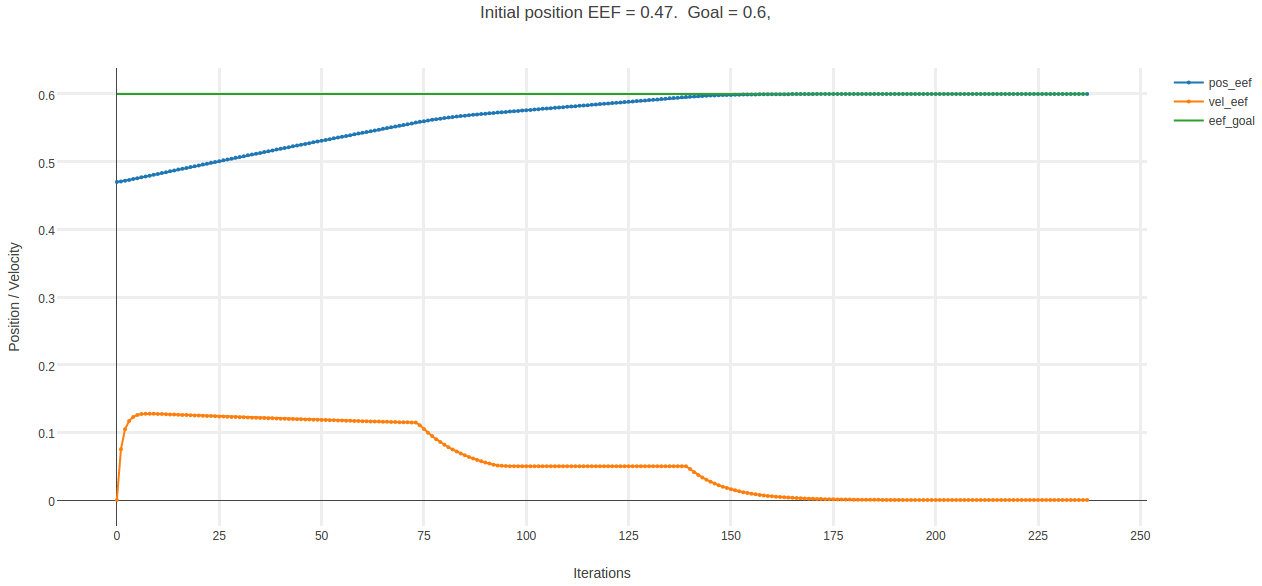
\includegraphics[width=0.75\linewidth, angle=0]{controllers/joint_eef.png}
	\vspace{-10pt}
	\caption[Joint and EEF goal: EEF trajectory]{Trajectory (dashed), velocity (continuous) and goal (dotted) of the EEF.}
	\vspace{-15pt}
	\label{fig:joint_eef}
\end{figure}
The initial position of the EEF is $0.47$, and of the joints $q_{0}= 0.02$ and $q_{0}= -0.15$, respectively. Only a goal for the EEF and for the first joint, $EEF_{f}= 0.6$ and $q_{0f} = -0.25$ are specified.

It can be seen in figure \ref{fig:joint_0} that one of the joints changes direction after around 75 iterations. This happens because the goal of the EEF and of the joint are in different directions, the system tries to minimize first the EEF error and afterwards the one of the joint.
\begin{figure}[H]
	\centering
	\begin{subfigure}[][Joint $q_{0}$]
		{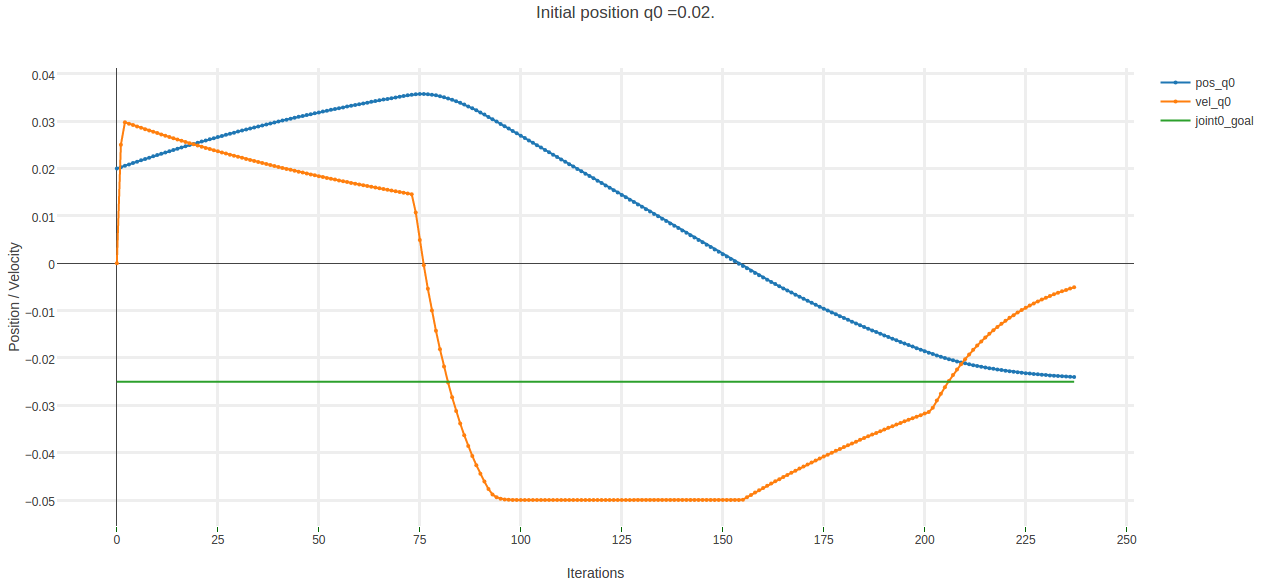
\includegraphics[width=0.49\linewidth]{controllers/joint_q0.png}}
	\end{subfigure}
	\begin{subfigure}[][Joint $q_{1}$]
		{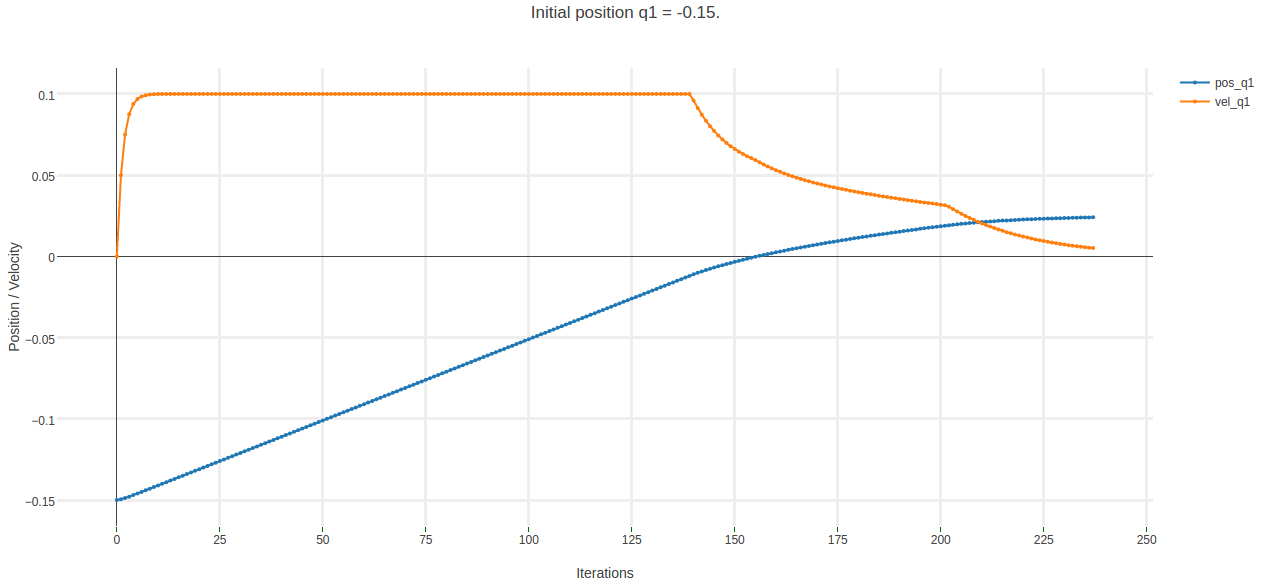
\includegraphics[width=0.49\linewidth]{controllers/joint_q1.png}}
	\end{subfigure}
	\vspace{-12pt}
	\caption[Joint and EEF goal: Joints Trajectories]{Trajectories (dashed) and velocities of both joints and goal (dotted) of $q_{0}$.}
	\vspace{-10pt}
	\label{fig:joint_0}
\end{figure}

 This behavior suggest  that it might be better to split the problem when goals for the joints are specified, where in the first part the joint goals are satisfied and kept constant and in the second part the EEF is reached.


\subsection{Position range as goal for the EEF}

In this example, the goal specified for the EEF is not one specific position, but a range, where any point in this area is a valid goal for the EEF.

Figure \ref{fig:range_1} shows the trajectory followed by the EEF while reaching the goal, it stops shortly after entering the given goal range. If a specific point inside this range is preferred as goal, an \textit{attractor} can be created,so that the EEF will try to reach the point defined by the attractor, if it is not possible, it will stay in the goal range.
\begin{figure}[H]
	\centering
	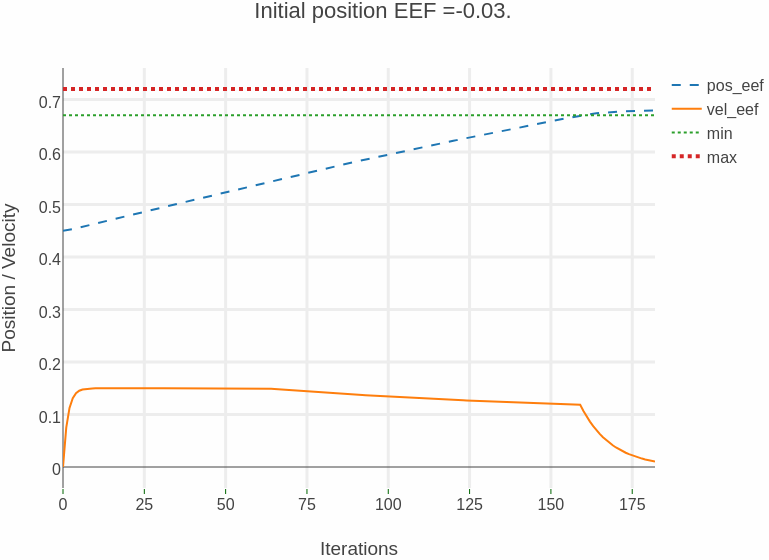
\includegraphics[width=0.8\linewidth, angle=0]{controllers/range_1.png}
	\vspace{-10pt}
	\caption[Position range as goal]{Trajectory (dashed) and velocity of the $EEF$, the goal range is between the dotted lines.}
	\vspace{-15pt}
	\label{fig:range_1}
\end{figure}

To achieve this behavior, matrix $\textbf{A}$ and it's limits, $\vec{lbA}$ and $\vec{ubA}$, are modified, rewriting equation \ref{eq:a_constr} as:
$$
\left( \begin{array}{c}
error \\
-q_{0,max} - q_{0} \\
-q_{1,max} - q_{1} \\
a_{0,min\_lim} \\
a_{1,min\_lim} \\
range_{min} - q_{eef}
\end{array}
\right)	\leq 
\left[ \begin{array}{cccc}
1 & 1 & 1 & 0 \\
1 & 0 & 0 & 0 \\
0 & 1 & 0 & 0 \\
1 & 0 & 0 & 0 \\
0 & 1 & 0 & 0 \\
1 & 1 & 0 & 1 \\
\end{array}
\right] *
\left( \begin{array}{c}
\dot{q}_{0} \\
\dot{q}_{1} \\
\epsilon \\
\epsilon_r \\
\end{array}
\right) 
\leq \left( \begin{array}{c}
error \\
q_{0,max} - q_{0} \\
q_{1,max} - q_{1} \\
a_{0,max\_lim} \\
a_{1,max\_lim} \\
range_{max} - q_{eef}
\end{array}
\right)
$$
\\
where $\epsilon_r$ is the slack factor for the goal range. The error is calculated using the attractor (goal) $error = attr - q_{eef}$. Here, the weight vector is defined as $\vec{\omega} = [ \omega_{1},\ \omega_{2},\ \omega_{3},\ \omega_{4} ]$. The constraints of the state vector (eq. \ref{eq:state_constr}) is rewritten as

$$
\left( \begin{array}{c}
-\dot{q}_{0,max} \\
-\dot{q}_{1,max} \\
-\epsilon_{max} \\
\epsilon_{r,max} \\
\end{array}
\right)	\leq 
\left[ \begin{array}{cccc}
\omega_{1} & 0 & 0 & 0 \\
0 & \omega_{2} & 0 & 0 \\
0 & 0 & \omega_{3} & 0 \\
0 & 0 & 0 & \omega_{4} \\
\end{array}
\right] *
\left( \begin{array}{c}
\dot{q}_{0} \\
\dot{q}_{1} \\
\epsilon \\
\epsilon_r \\
\end{array}
\right) 
\leq \left( \begin{array}{c}
\dot{q}_{0,max} \\
\dot{q}_{1,max} \\
\epsilon_{max} \\
\epsilon_{r,max} \\
\end{array}
\right)
$$
\\
where $\omega_{1}$ and $\omega_{2}$ are the joint's weights, $\omega_{3}$ is the weight of the attractor, and $\omega_{4}$ is the weight of the goal range.
 
Figures \ref{fig:range_eef} to \ref{fig:range_q1} show the behavior of the EEF and joints. In this example, the attractor was set at $0.7$ with the range between $0.67$ and $0.72$. It can be seen how the EEF reaches the goal set by the attractor, instead of just staying at the range borders. 

\begin{figure}[H]
	\centering
	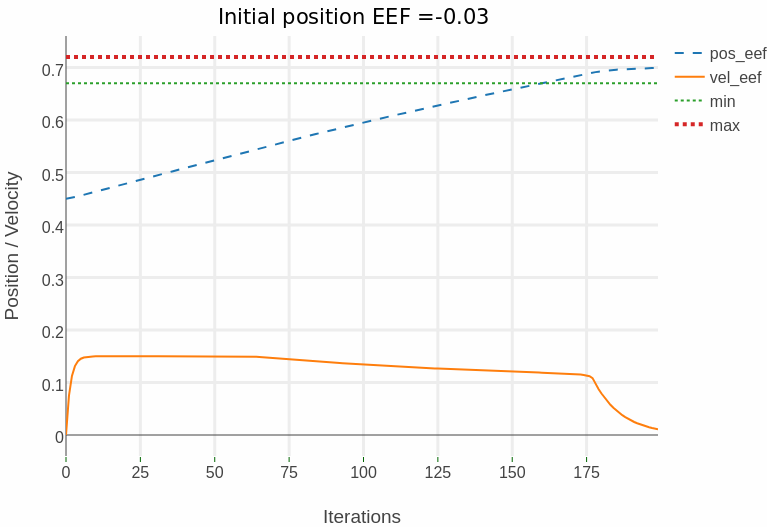
\includegraphics[width=0.8\linewidth, angle=0]{controllers/range_eef.png}
	\vspace{-10pt}
	\caption[Position range with attractor: EEF]{Trajectory (dashed) and velocity of the EEF, here an attractor is defined inside the range.}
	\vspace{-15pt}
	\label{fig:range_eef}
\end{figure}
\begin{figure}[H]
	\centering
	\begin{subfigure}[][Joint $q_{0}$]
		{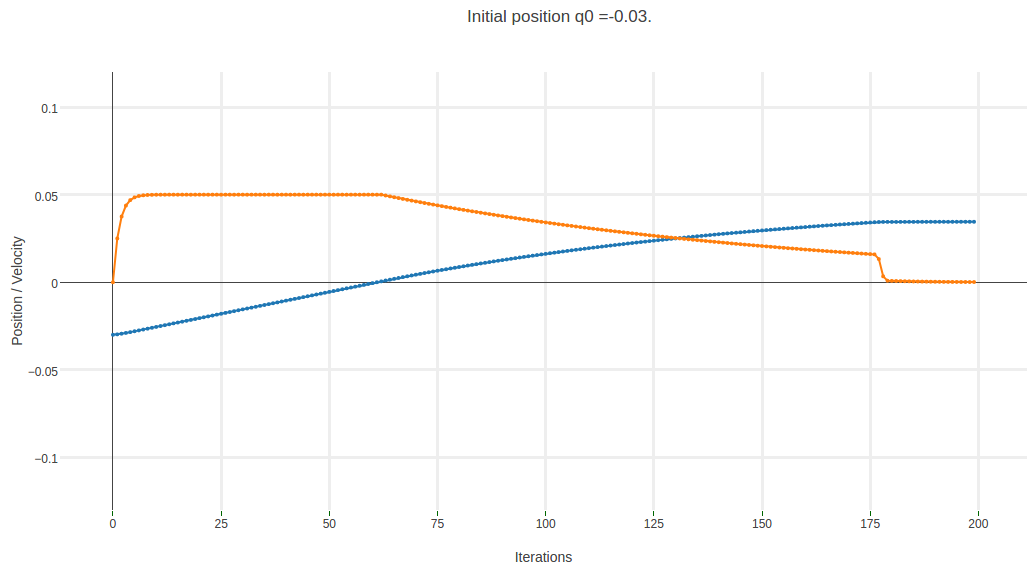
\includegraphics[width=0.49\linewidth]{controllers/range_q0.png}}
	\end{subfigure}
	\begin{subfigure}[][Joint $q_{1}$]
		{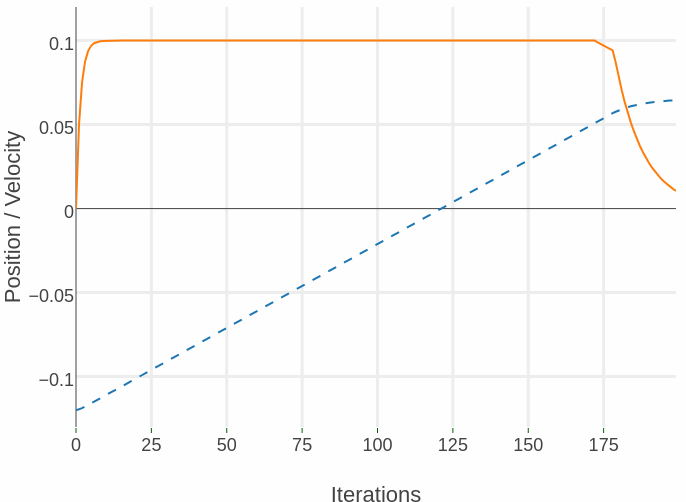
\includegraphics[width=0.49\linewidth]{controllers/range_q1.png}}
	\end{subfigure}
	\vspace{-12pt}
	\caption[Position range with attractor: Joints]{Trajectory (dashed) and velocity of both joints. Each joint has a different velocity and acceleration constraint, as well as different joint limits.}
	\vspace{-10pt}
	\label{fig:range_q1}
\end{figure}
The weight of the attractor is set higher than the range's weight, this means that the cost of reaching the point defined by the attractor is higher than just going inside the range. By doing this, the optimization algorithm prioritizes moving the EEF to the given range. Modifying these weights determine how close will the EEF come to the attractor.

\subsection{Multiple goals for the EEF}

It is also possible to specify multiple goals for the EEF and select one of them using the weights assigned to each goal. This controller shows a two DOF  linear manipulator where two goals are specified. In this case, the matrix \textbf{A} and it's limits (given by equation \ref{eq:a_constr}) are given by:

$$
\left( \begin{array}{c}
error_{goal1} \\
error_{goal2} \\
-q_{0,max} - q_{0} \\
-q_{1,max} - q_{1} \\
a_{0,min\_lim} \\
a_{1,min\_lim} \\
\end{array}
\right)	\leq 
\left[ \begin{array}{cccc}
1 & 1 & 1 & 0 \\
1 & 1 & 0 & 1 \\
1 & 0 & 0 & 0 \\
0 & 1 & 0 & 0 \\
1 & 0 & 0 & 0 \\
0 & 1 & 0 & 0 \\
\end{array}
\right] *
\left( \begin{array}{c}
\dot{q}_{0} \\
\dot{q}_{1} \\
\epsilon_1 \\
\epsilon_2 \\
\end{array}
\right) 
\leq \left( \begin{array}{c}
error_{goal1} \\
error_{goal2} \\
q_{0,max} - q_{0} \\
q_{1,max} - q_{1} \\
a_{0,max\_lim} \\
a_{1,max\_lim} \\
\end{array}
\right)
$$

where $\epsilon_1$ and $\epsilon_2$ are the slack factors for the first  and second goal, respectively. The weight vector is defined as $\vec{\omega} = [ \omega_{1},\ \omega_{2},\ \omega_{3},\ \omega_{4} ]$. Where $\omega_{1}$ and $\omega_{2}$ are the joint's weights, $\omega_{3}$ and $\omega_{4}$ are the goals' weight. The constraints of the state vector (eq. \ref{eq:state_constr}) is rewritten as:

$$
\left( \begin{array}{c}
-\dot{q}_{0,max} \\
-\dot{q}_{1,max} \\
-\epsilon_{1,max} \\
\epsilon_{2,max} \\
\end{array}
\right)	\leq 
\left[ \begin{array}{cccc}
\omega_{1} & 0 & 0 & 0 \\
0 & \omega_{2} & 0 & 0 \\
0 & 0 & \omega_{3} & 0 \\
0 & 0 & 0 & \omega_{4} \\
\end{array}
\right] *
\left( \begin{array}{c}
\dot{q}_{0} \\
\dot{q}_{1} \\
\epsilon_1 \\
\epsilon_2 \\
\end{array}
\right) 
\leq \left( \begin{array}{c}
\dot{q}_{0,max} \\
\dot{q}_{1,max} \\
\epsilon_{1,max} \\
\epsilon_{2,max} \\
\end{array}
\right)
$$
\\
In the first example, two goals are specified but only the first one is selected using the goal's weights. Goal one, located at $q_{des1} = 0.55$, has a weight of $\omega_{3} = 0.1$ and the second goal, located at $q_{des2} = 0.75$, has a weight of $\omega_{4} = 0.001$, the initial position of the EEF is at $q_{eef} = 0.7$. As shown in figure \ref{fig:goal1}(a), the EEF reaches the first goal (thick dotted line).

\begin{figure}[H]
	\centering
	\begin{subfigure}[First Goal]
		{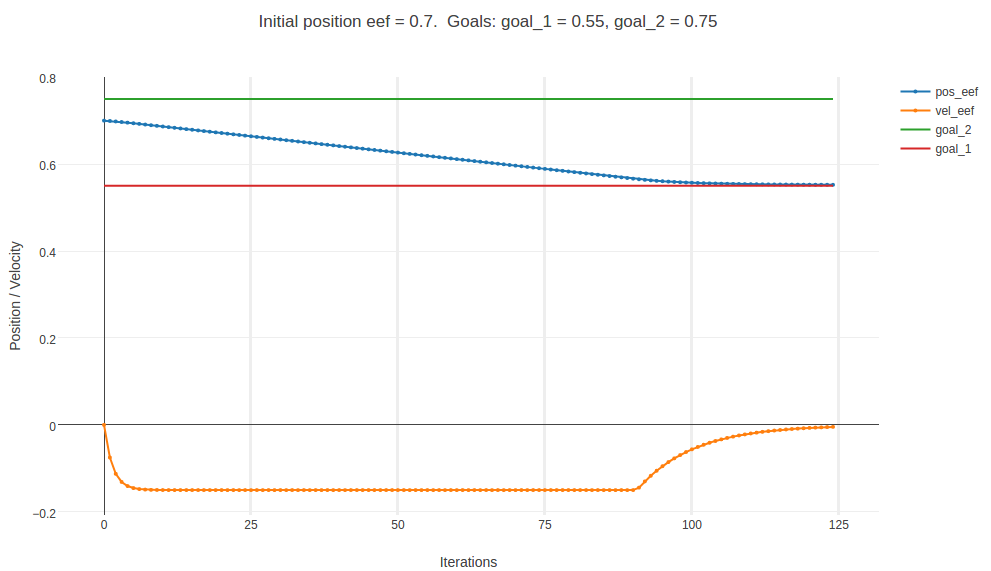
\includegraphics[width=0.49\linewidth]{controllers/multip_1.png}}
	\end{subfigure}
	\begin{subfigure}[Second goal]
		{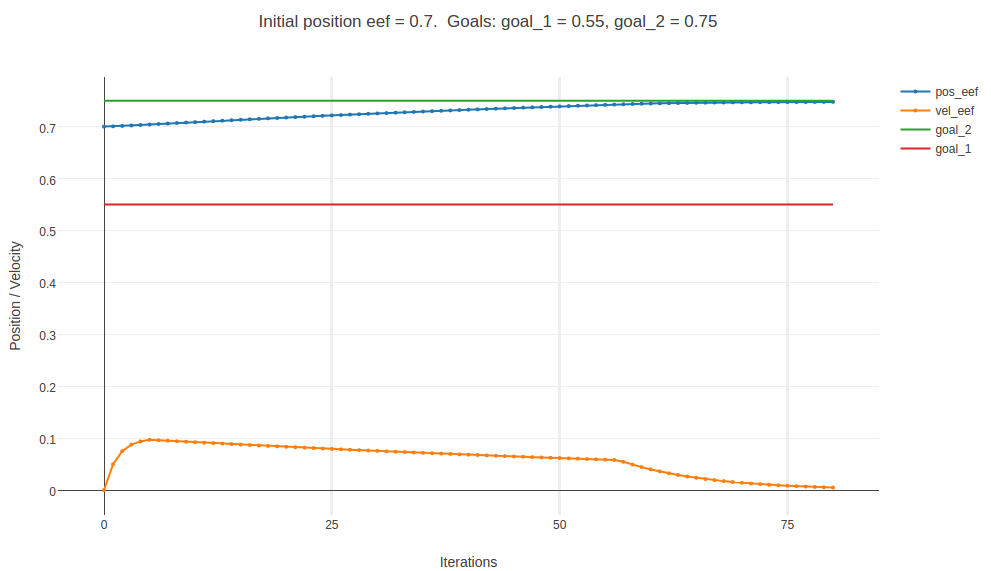
\includegraphics[width=0.49\linewidth]{controllers/multip_2.png}}
	\end{subfigure}
	\vspace{-12pt}
	\caption[Multiple goals]{The selected goal changes depending on the weights. Trajectory (dashed) and velocity of the EEF.}
	\vspace{-10pt}
	\label{fig:goal1}
\end{figure}

By inverting the weights, $\omega_{3} = 0.001$ and $\omega_{4} = 0.1$, the active goal changes (figure \ref{fig:goal1} (b)). It can be seen that the velocity of the EEF in figure \ref{fig:goal1} (b) is lower than in (a). This is caused due to the proximity of one of the joints to the joint limit, which was reached shortly after 50 iterations.

It is possible to make the EEF reach a point between both goals, by setting similar or equal weights to both goals (figure \ref{fig:goal2}). 
\begin{figure}[H]
	\centering
	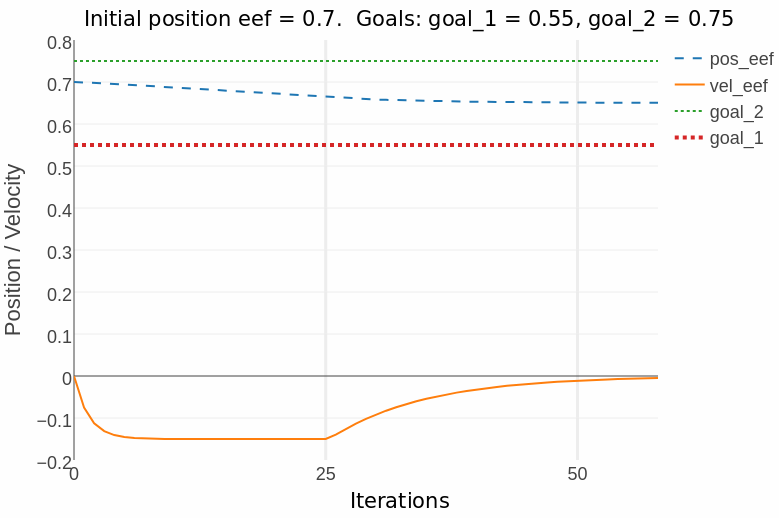
\includegraphics[width=0.6\linewidth, angle=0]{controllers/multip_3.png}
	\vspace{-10pt}
	\caption[Multiple goals: Middle point]{Trajectory (dashed) and velocity  of the EEF. Same weight in both goals. Each joint has a different velocity and acceleration constraint, as well as different joint limits.}
	\vspace{-15pt}
	\label{fig:goal2}
\end{figure}
If the weight of both goals is similar, the EEF will stay closer to one goal, without reaching it. Selecting the appropriate weight combination, any point between both goals can be reached.


\subsection{Dynamic weights}

It is possible to automatically select between two goals using dynamic weights, which change with the distance. This controller calculates the weight of each goal in every iteration, with the error to the goals $q_{des1}$ and $q_{des2}$ as: 
$$error_1 = (q_{des1} - q_{eef})*p $$
and
$$error_2 = (q_{des2} - q_{eef})*p $$

where $p$ is the proportional gain and $q_{eef}$ the current position of the EEF. The weights are calculated with:
\begin{subequations}
	\begin{align}
		 \omega_3 = \left( \dfrac{error_2}{error_1 + error_2} \right) ^{2} \\
		 \omega_4 = \left( \dfrac{error_1}{error_1 + error_2} \right) ^{2}
	\end{align}
	\label{eq:dyn}
	\vspace{-10pt}
\end{subequations}

The controller will then select the closest goal, which gets a higher weight. 

In this example, the initial position of the EEF is set between both goals. The first goal is set at $0.45$ and the second one at $0.78$. As shown in figure \ref{fig:dynamic}, the EEF reaches the closest goal. The only parameter changed between figure \ref{fig:dynamic} (a) and (b) is the EEF's initial position. 
\begin{figure}[H]
	\centering
	\begin{subfigure}[EEF closer to goal 2 (thick dotted line)]
		{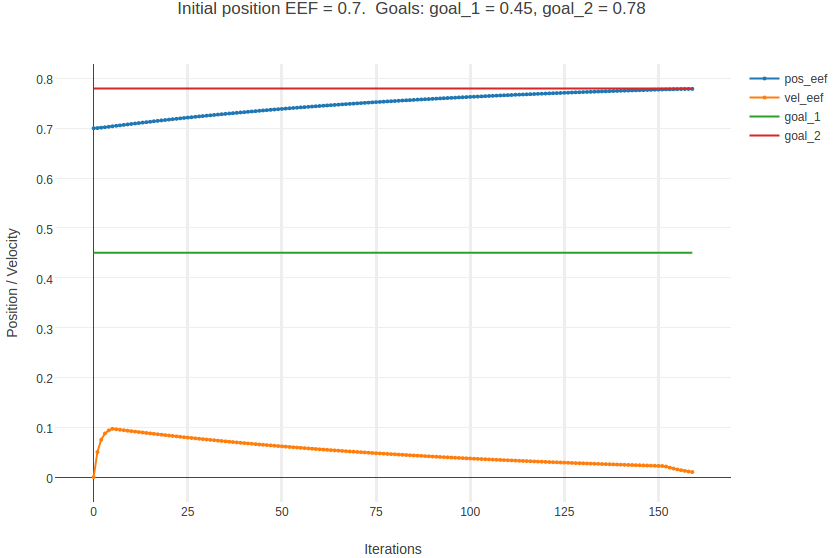
\includegraphics[width=0.49\linewidth]{controllers/dynamic_1.png}}
	\end{subfigure}
	\begin{subfigure}[EEF closer to goal 1 (thin dotted line)]
		{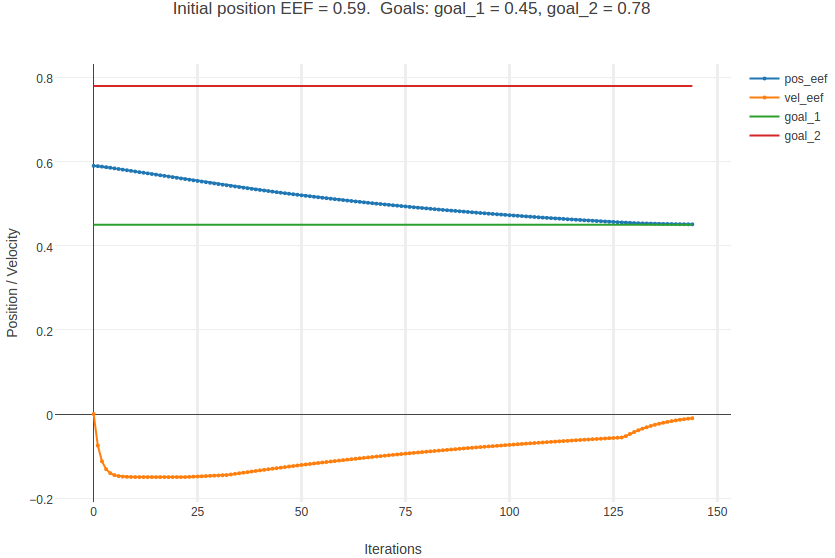
\includegraphics[width=0.49\linewidth]{controllers/dynamic_2.png}}
	\end{subfigure}
	\vspace{-12pt}
	\caption[Dynamic weights: EEF]{The selected goal changes depending on the initial position of the EEF, weights are calculated on every iteration. Trajectory (dashed) and velocity of the EEF.}
	\vspace{-10pt}
	\label{fig:dynamic}
\end{figure}

\begin{figure}[H]
	\centering
	\begin{subfigure}[Joint $q_0$]
		{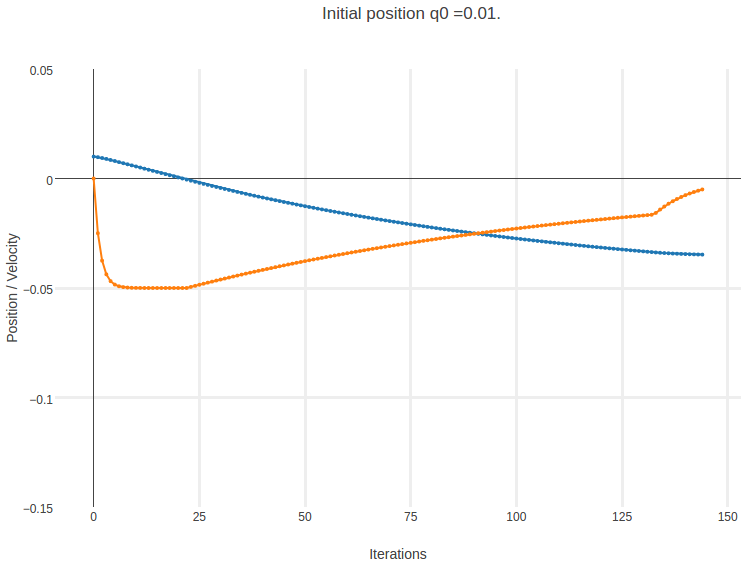
\includegraphics[width=0.49\linewidth]{controllers/dynamic_3.png}}
	\end{subfigure}
	\begin{subfigure}[Joint $q_1$]
		{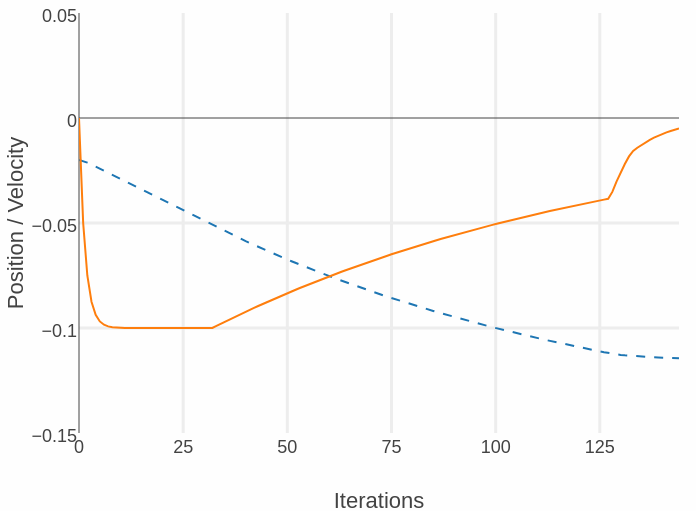
\includegraphics[width=0.49\linewidth]{controllers/dynamic_4.png}}
	\end{subfigure}
	\vspace{-12pt}
	\caption[Dynamic weights: Joints]{Trajectories (dashed) and velocities of both joints. Each joint has a different velocity and acceleration constraint, as well as different joint limits.}
	\vspace{-10pt}
	\label{fig:dynamic_j}
\end{figure}

Figure \ref{fig:dynamic_j} shows the trajectories followed by both joints in the second example (\ref{fig:dynamic} (b)). It can be seen that the velocity profile of both joints are similar. The difference in scale is due to the velocity constraints each joint has.

\subsection{Three goals for the EEF}

A problem seems to appear if dynamic weights are calculated when three or more goals are specified. Taking three goals as an example, if two of them are close together ($q_{des2}$ and $q_{des3}$), the controller will ignore the third goal ($q_{des1}$) and reach for a point between the other two goals, since minimizing two errors is better (mathematically speaking) than one.

This problem can be solved by modifying the formula used to calculate the goal's weights, so we can rewrite equation \ref{eq:dyn} as:
\begin{subequations}
	\begin{align}
		\omega_3 = \left(\dfrac{1 - \rvert error_1 - error_{min} \rvert}{error_{max} + error_{min}}\right)^{3} \\
		\omega_4 = \left(\dfrac{1 - \rvert error_2 - error_{min} \rvert}{error_{max} + error_{min}}\right)^{3} \\
		\omega_5 = \left(\dfrac{1 - \rvert error_3 - error_{min} \rvert}{error_{max} + error_{min}}\right)^{3} 
	\end{align}
\end{subequations}
where:
$$error_{min} = min(\rvert error_1\rvert, \rvert error_2\rvert, \rvert error_3\rvert)\vspace{-10pt}$$ 
$$error_{max} = max(\rvert error_1\rvert, \rvert error_2\rvert, \rvert error_3\rvert)$$
The matrix \textbf{A} and it's limits as well as the state vector are extended to fit the extra goals:
$$
\left( \begin{array}{c}
error_{1} \\
error_{2} \\
error_{3} \\
-q_{0,max} - q_{0} \\
-q_{1,max} - q_{1} \\
a_{0,min\_lim} \\
a_{1,min\_lim} \\
\end{array}
\right)	\leq 
\left[ \begin{array}{ccccc}
1 & 1 & 1 & 0 & 0 \\
1 & 1 & 0 & 1 & 0 \\
1 & 1 & 0 & 0 & 1 \\
1 & 0 & 0 & 0 & 0 \\
0 & 1 & 0 & 0 & 0 \\
1 & 0 & 0 & 0 & 0 \\
0 & 1 & 0 & 0 & 0 \\
\end{array}
\right] *
\left( \begin{array}{c}
\dot{q}_{0} \\
\dot{q}_{1} \\
\epsilon_1 \\
\epsilon_2 \\
\epsilon_3 \\
\end{array}
\right) 
\leq \left( \begin{array}{c}
error_{1} \\
error_{2} \\
error_{3} \\
q_{0,max} - q_{0} \\
q_{1,max} - q_{1} \\
a_{0,max\_lim} \\
a_{1,max\_lim} \\
\end{array}
\right)
$$

Two examples in figure \ref{fig:dynamic3} show the behavior of this controller

\begin{figure}[H]
	\centering
	\begin{subfigure}[EEF closer to goal 2 (dotted)]
		{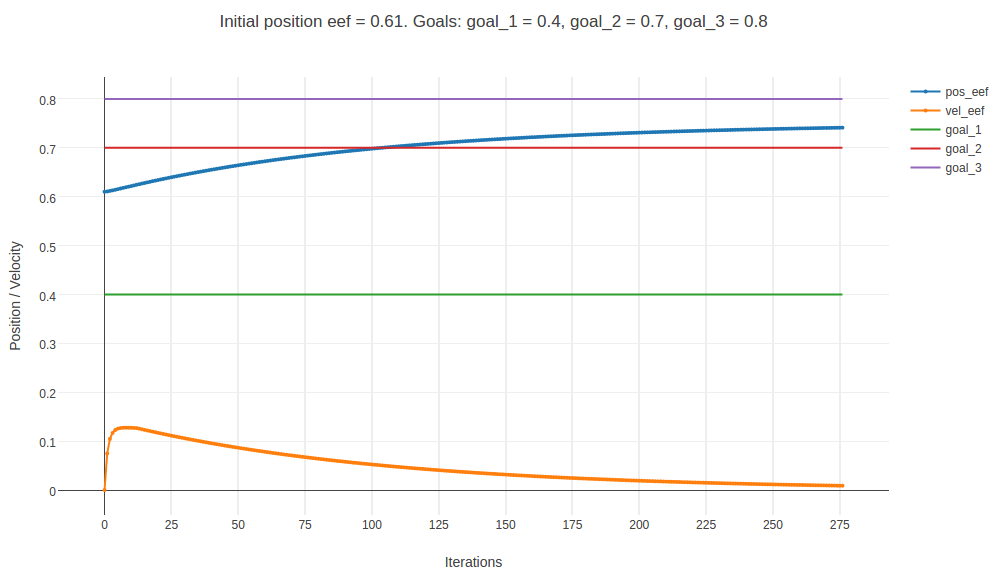
\includegraphics[width=0.48\linewidth]{controllers/dyn_3_eef_1.png}}
	\end{subfigure}
	\begin{subfigure}[EEF closer to goal 1 (thin dotted)]
		{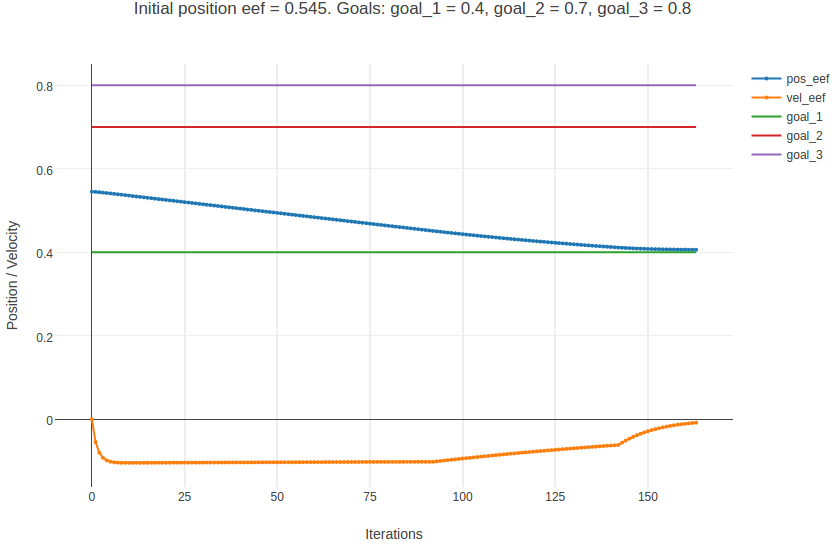
\includegraphics[width=0.48\linewidth]{controllers/dyn_3_eef_2.png}}
	\end{subfigure}
	\vspace{-2pt}
	\caption[Dynamic weights: EEF]{The selected goal changes depending on the initial position of the EEF. Trajectory (dashed) and velocity of the EEF.}
	\vspace{-15pt}
	\label{fig:dynamic3}
\end{figure}
The controller does not always reach a goal, as seen in figure \ref{fig:dynamic3} (a), if two of the given goals are close together, the EEF will stay between both.This can still be implemented as a controller for a robot if the goals are grasping poses of an object, since the gripper will still reach out for the object and in some cases a point between grasping poses can also be used to grasp the object, like when grasping a box.

The code generated for this controllers can be downloaded from Github\footnote{https://github.com/mgvargas/qpOASES}.

\subsection{Robot controller}

A controller with the same structure as the ones shown in the previous subsections was developed for the Boxy robot. Boxy's geometry and kinematics are taken from the URDF file (section \ref{sec:urdf}). 

The definition of the matrix \textbf{A} and of the state vector $\ \vec{s}\ \in\ \Re^{nV}$ changes due to the DOF's and kinematics of the robot, so equation \ref{eq:state} changes to:
\begin{equation}
\vec{s} = [\dot{\ q_{0}} \ \ \dot{q_{1}} \ ... \dot{q_{C}} \ \ \epsilon_{0} ... \ \epsilon_{6} ]^{T}
\end{equation}
where $\dot{q_{0}}$ to $\dot{q_{C}}$ are the joints velocities, three for the base, one for the torso and seven for the arm, and $\epsilon_{0}$ to $\epsilon_{6}$ are slack variables, one per DOF. The matrix $\textbf{A} \in \Re^{nC\times nV}$ is defined using the Jacobian:
\begin{equation}
\textbf{A} =
\left[ \begin{array}{cc}
\textbf{J} & \textbf{I}_{p,p} \\
\textbf{I}_{m,m} & \textbf{0}_{m,p} \\
\textbf{I}_{m,m} & \textbf{0}_{m,p} \\
\end{array}
\right]
\end{equation}
where $\ \textbf{J}\ \in\ \Re^{p\times m}$ is the Jacobian, $\ \textbf{I}$ is the identity matrix, $\ \textbf{0}$ is a zero matrix, $p$ is the number of DOF and $m$ the number of joints to control. The constraint vectors are created using the error, joint limits and acceleration constraints:
\begin{subequations}
	\begin{align}
		\vec{lbA} = [\ \vec{error}_{pos},\ \vec{error}_{orient},\ -\vec{q}_{max} - 	\vec{q},\ \vec{a}_{min\_lim} ]^{T}\\
		\vec{ubA} = [\ \vec{error}_{pos},\ \vec{error}_{orient},\ \vec{q}_{max} - \vec{q},\ \vec{a}_{max\_lim} ]^{T}
	\end{align}
	\label{eq:const_vectors}
\end{subequations}
where the acceleration limit is calculated using equation \ref{eq:accel}, $\ \vec{q}_{max}$ is the vector of joint limits and $\vec{q}$ the current position of the joints. The $\vec{error}_{pos}$ is the position error and $\vec{error}_{orient}$ the orientation error. 

The position error is calculated  considering a proportional gain, to accelerate the convergence of the system:
$$\vec{error}_{pos} = (\vec{q}_{des} - \vec{q}_{eef})*p $$
where $\vec{q}_{des}$ is the goal position, $\vec{q}_{eef}$ the current position of the EEF and $p$ is the proportional gain. 

However, calculating the orientation error cannot be done by simply subtracting goal orientation from the current one. Several approaches for solving this problem are explained by \cite{siciliano}. In this work, the orientation error is calculated using quaternion \textit{spherical linear interpolation} (Slerp). The Slerp gives an interpolation between 0 and 1 from the given quaternions. It was developed by \cite{slerp}:
$$ Slerp(t;q_0,q_1)=\dfrac{q_0\sin((1-t)\theta) + q_1\sin(t\theta)}{\sin\theta} 
$$
for $0\ \leq \ t\ \leq 1$. Using Slerp, it was possible to calculate an orientation error for the system set as goal for every iteration a small part of the total error. Using the quaternion obtained by the Slerp, the error can be calculated, as explained by \cite{siciliano}, as:
$$ q_{error} = q_{goal} * q_{current}^{-1} $$
The Algorithm 2 is used to calculate the error and the obtained quaternion is transformed to euler angles and given as $\vec{error}_{orient}$ to the constraint vectors \ref{eq:const_vectors}.
\begin{algorithm}[t!]
	\caption{Orientation Error using Slerp}\label{algor:error}
	\begin{algorithmic}[1]
		\vspace{2pt}
		\State $q_{whole\_error} = q_{goal} *\ q_{eef}^{-1}$;
		\vspace{2pt}
		\State $rot_{vector} = quat\_to\_axisangle(\ q_{whole\_error})$;
		\vspace{3pt}
		\State $rot_{error}  = \sqrt{rot_{vector}[0]^{2} + rot_{vector}[1]^{2} + rot_{vector}[2]^{2}}$
		\vspace{3pt}
		\If{$\ t = threshold - rot_{error} \geq 0\ $} 
		\vspace{2pt}
		\State $t = 1$;
		\vspace{1pt}
		\Else 
		\State $threshold / rot_{error}$;\EndIf
		\vspace{1pt}
		\State $q_{interpolation} = Slerp\ (t;q_{eef},q_{goal})$;
		\vspace{1pt}
		\State $q_{error} = q_{interpolation} *\ q_{eef}^{-1}$;
		\vspace{-1pt}
	\end{algorithmic}
\end{algorithm}


The weight vector $\ \vec{\omega}$ is calculated on every iteration and used to update matrix $\textbf{H}$, which is used to calculate the cost in equation \ref{eq:cost}. 
\begin{equation}
	\textbf{H}\ =\ diag(\vec{\omega})
	\label{eq:h}
\end{equation}

The value of the weights depends on the distance between the robot and the goal, the calculations are explained in algorithm \ref{algor:weight}. Where $distance$ is the distance between the EEF and the goal, $weight_{active}$ and $weight_{inactive}$ are constant values, $weight_{active} \ll weight_{inactive}$, $far$ and $near$ are threshold distances.

\begin{algorithm}[t!]
	\caption{Dynamic weight calculation}\label{algor:weight}
	\begin{algorithmic}[1]
		\vspace{2pt}
		\If {$\ distance\ \geq far\ $}
		\vspace{2pt}
		\State $weights_{base} = weight_{active}$;
		\State $weight_{torso} = weight_{active}$;
		\vspace{2pt}
		\For {n in joints}
		\State $weights_{arm}[n] = weight_{inactive}$;
		\EndFor
		\ElsIf {$\ near \leq pos_{robot}\ \leq far\ $}
		\vspace{3pt}
		\For {n in joints}
		\State $weights_{arm}[n] = \dfrac{(weight_{inactive} - weight_{active})*(distance - near)}{far - near} + weight_{active}$;
		\EndFor
		\State $weights_{base} = \dfrac{(weight_{active} - weight_{inactive})*(distance - near)}{far - near} + weight_{inactive}$;
		\State $weight_{torso} = weights_{base}$;
		\Else
		\vspace{2pt}
		\State $weights_{base} = weight_{inactive}$;
		\vspace{2pt}
		\State $weight_{torso} = \dfrac{(weight_{active} - weight_{inactive})*(abs(error_{pos}[2]))}{far} + weight_{inactive}$;
		\For {n in joints}
		\vspace{2pt}
			\State $weights_{arm}[n] = weight_{active}$;
		\EndFor
		\EndIf
		\vspace{-1pt}
	\end{algorithmic}
\end{algorithm}

If the robot is too far away from the given goal, the arm joints are disabled and only the base moves. Between a certain distance threshold, both base and arms can move, with the weights dynamically changing in accordance to the distance. If the robot is close to the goal, only the arms and torso are allowed to freely move, the weight of the base is increased so that the controller prefers moving arms and torso to base.
\begin{figure}[H]
	\centering
	\begin{subfigure}[][Isometric view]
		{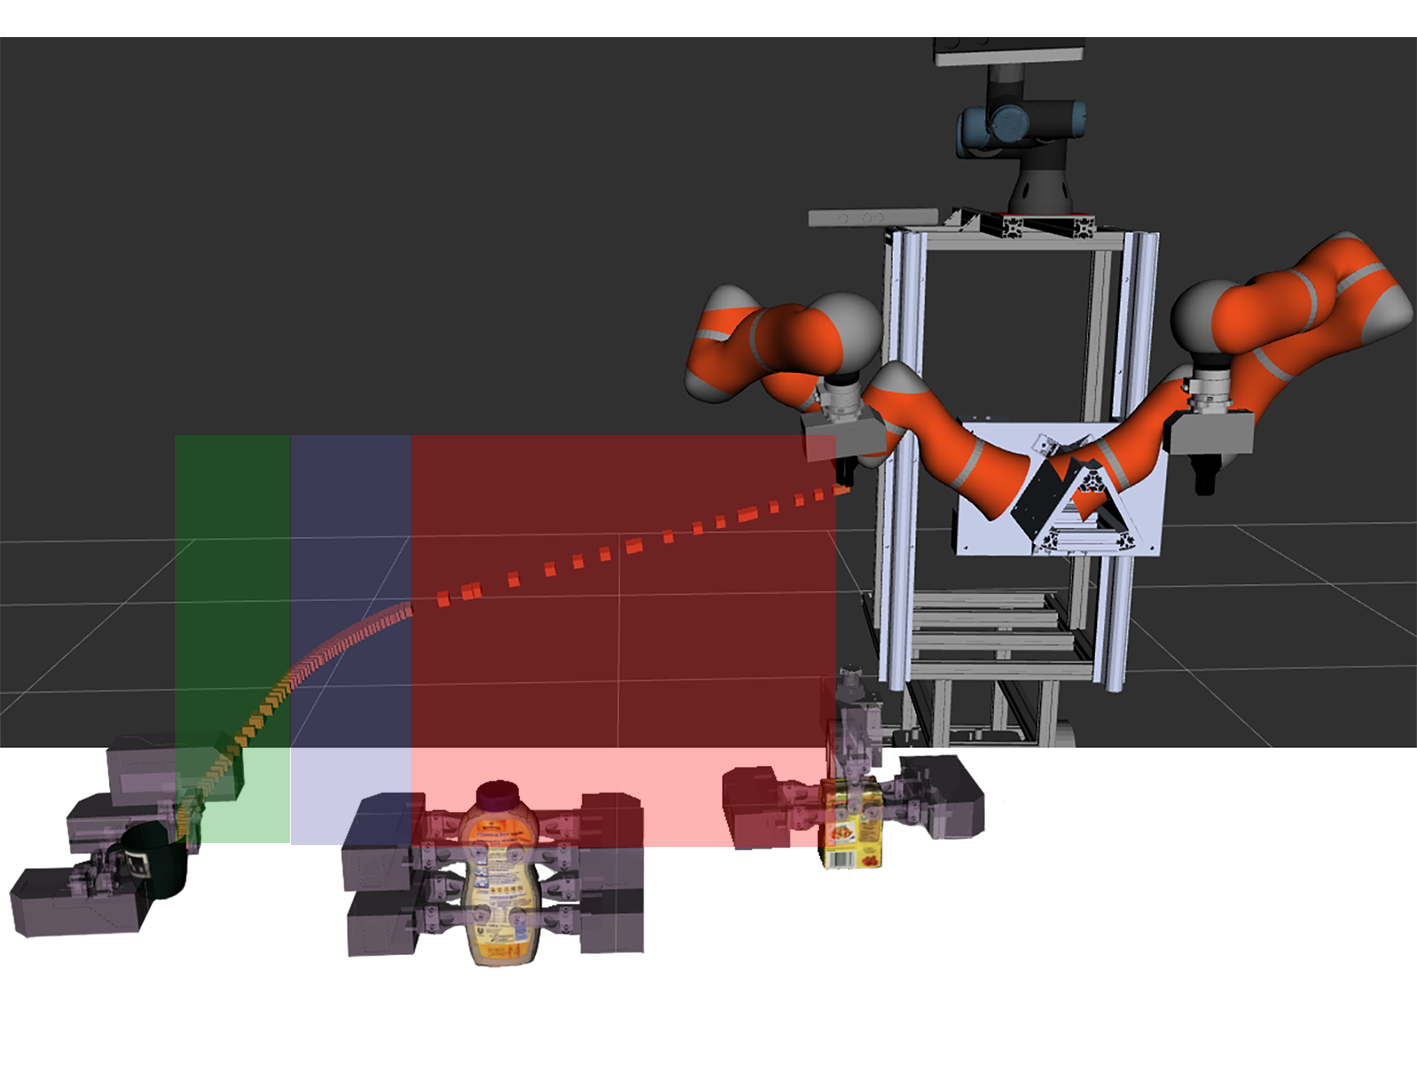
\includegraphics[width=0.41\linewidth]{boxy/Trajectory01.png}}
	\end{subfigure}
	\begin{subfigure}[][Top view]
		{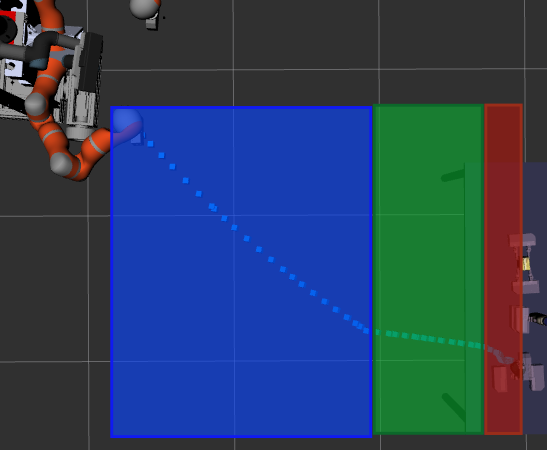
\includegraphics[width=0.4\linewidth]{boxy/TrajectoryParts.png}}
	\end{subfigure}
	\vspace{-10pt}
	\caption[Boxy's Trajectory]{Trajectory (dashed) of the EEF. The weights are calculated on every iteration.}
	\vspace{-15pt}
	\label{fig:traj1}
\end{figure}

Figure \ref{fig:traj1} shows a simulated trajectory followed by the EEF while reaching out for a cup. The right area in figure \ref{fig:traj1} (b) shows the part of the trajectory where mainly the base was moved, the middle area is where arms, torso and base were active and the left area is where mainly the arm and torso were used.

The first goal set to the controller is a pre-grasping pose, located three centimeters away on the Z-axis from the current grasping pose. Once the EEF is within a certain position and orientation threshold from the  pre-grasping pose, it moves towards the final grasping pose. The pre-grasping pose is defined to help avoiding collisions with the object, the EEF can approach the object only when the orientation is already correct and will do so in a way that it will not try to go through the object in order to reach the grasping pose.

\section{Trajectory Evaluation}
\label{sec:traj_eval}

When the projection manager system receives a request to grasp an object, it asks the controller for several trajectories. The trajectory evaluation service is in charge of assigning scores to each one on these trajectories and sending the best one back.

First, each trajectory is sent to the \textit{collision detection} node, if a collision is found, the trajectory gets discarded, if not, the minimum distance between the robot and an object is obtained. The remaining trajectories are then evaluated.

For the evaluation, different metrics are considered
\begin{itemize}
	\item Length of the generated path
	\item Smoothness: No abrupt changes in velocity and acceleration
	\item Convergence error: How far was the arm from the desired position
	\item Manipulability of the EEF after reaching the goal
	\item Distance to collision: Minimum distance from the arm to any object in the scene
\end{itemize}


The manipulability is calculated as proposed by \cite{Yoshikawa}, who defines it as a quality measure for redundant manipulators, it describes the distance to singular configuration of the robot.
$$
manipulability = \sqrt{det(\textbf{JJ}^{T})}
$$
where $\textbf{J}$ is the Jacobian of the kinematic chain used to perform the trajectory. This approach was also used by \cite{manip_analysis}, they combine the manipulability with a penalization term that considers the distance to the joint limits to measure the robot's ability to maneuver in the workspace.

After simulation several experiments, a maximum value for acceleration and velocity change was defined, as well as for manipulability. The maximum length of the trajectory was obtained based on the robot arm workspace. Using these values, a score for each trajectory can be calculated:
\begin{equation}
\begin{aligned}
score = &\ w_l\frac{traj\_length}{max\_length}\ +\ w_v\frac{vel\_change}{max\_vel\_change}\ +\ w_a\frac{acc\_change}{max\_acc\_change} \\
 & \ +\ w_c\frac{collision\_distance}{min\_col\_distance} 
\ +\ w_e\frac{position\_error}{max\_position\_error}\\
 & \ +\ w_m(max\_manip\ -\ manipulability)
\end{aligned}
\label{eq:score}
\end{equation}


where $w_l$, $w_v$, $w_a$, $w_c$, $w_e$ $w_m$ are the weights for length, velocity change, acceleration change, distance to collision, convergence error and manipulability, respectively.

The trajectory with the lowest score is selected and sent back to the \textit{projection\_manager}, which sends it as a result to a PI controller. This controller sends the required commands to the robot to execute the trajectory.


\section{Collision Checking}
\label{sec:collision}
Since the motion controller is not able to detect collision objects in the environment, it is important to evaluate if the obtained trajectory would generate a collision if executed. To do so, the collision detection functionality of \textit{Moveit! Planning Scene} (section \ref{subsec:moveit}) was used. All objects detected by perception, as well as the collision model of the robot were loaded in a planning scene. The robot's URDF (section \ref{sec:urdf}) is also added to the planning scene, this allows to evaluate if the robot is in a valid state (feasibility) and to calculate the state of the robot given the joint values.

The object the robot will grasp is removed from the collision objects, since the grasping would be considered as a collision. This has the disadvantage that the robot's EEF might hit the object while reaching for the grasping pose and the collision detection would not perceive it. In order to reduce the possibility of this collision, a pre-grasping pose is set as initial goal for the EEF, this pose is located 3 cm away from the object. Only after the EEF has reached the pre-grasing pose, it approaches to the object.

For every step in the trajectory, the new joint values are loaded in the robot model. The planning scene evaluates if the robot is in a valid state and if there is any collision, both self-collisions and collisions with the environment are considered. If no collision was found, the minimum distance to an object is stored. The evaluation stops if a collision is found and the trajectory is discarded.

\section{PI Controller}
\label{sec:pi_controller}

The Boxy robot moves by receiving a sequence of velocity commands for the joints. This means: if the robot receives the command "move the base at $0.5\frac{m}{sec}$" during 2 seconds, it will execute this movement for two seconds. Therefore it is not possible to send a whole trajectory at once and expect the robot to move, since the trajectory is a sequence of desired positions and velocities.

The proportional and integral controller (PI controller) reads the trajectory step by step and sends the specified position for each joint. It reads the time stamps of the trajectory to find out where the robot should be after a certain time interval. It uses a proportional gain and an integral gain to compensate for the robot's inertia. 

The \textit{naive\_kinematic\_simulator} (section \ref{sub:naive}) used to generate the trajectories assumes that the robot will instantaneously execute the received commands and reached the desired speed. In reality, the robot needs some time to reach a certain speed due to inertia. The motion controller tries to consider this delay by setting acceleration limits while calculating the trajectories, but it stills needs some help from the PI controller to make the robot follow the desired trajectory.

\begin{figure}[H]
	\centering
	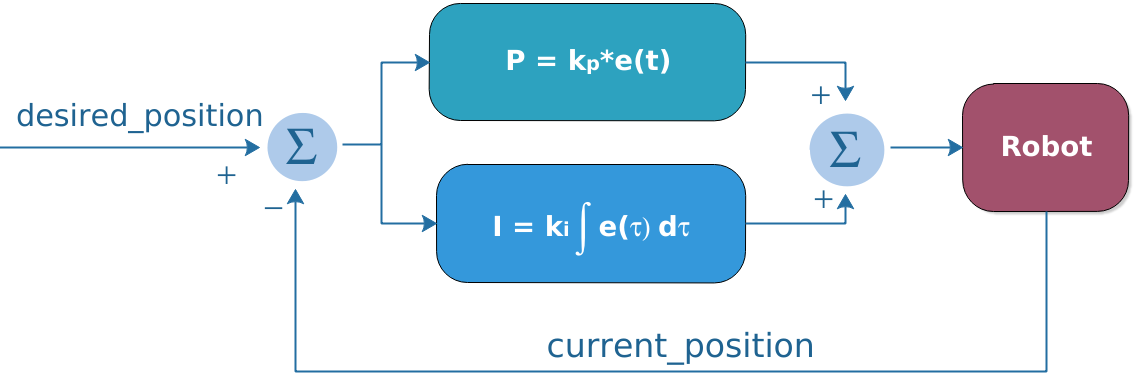
\includegraphics[width=0.8\linewidth]{pi_controller.png}
	\vspace{-10pt}
	\caption{Diagram of PI Controller}
	\vspace{-15pt}
	\label{fig:pi}
\end{figure}

Figure \ref{fig:pi} shows the diagram of the used PI controller. It was tuned to work with the Boxy robot first by tunning it with the \textit{naive\_kinematic\_simulator} and afterwards with the real robot.

\begin{figure}[H]
	\centering
	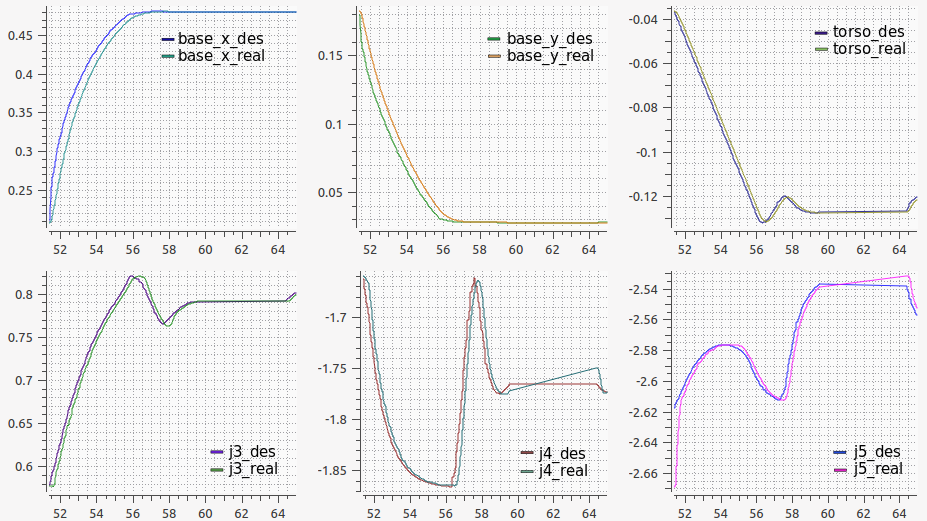
\includegraphics[width=0.99\linewidth]{pi_behavior1.png}
	\vspace{-10pt}
	\caption[Comparison: Generated and Executed trajectory]{Comparison between generated and executed trajectories. X axis - seconds, Y axis - joint values}
	\vspace{-15pt}
	\label{fig:behavior}
\end{figure}
\begin{figure}[H]
	\centering
	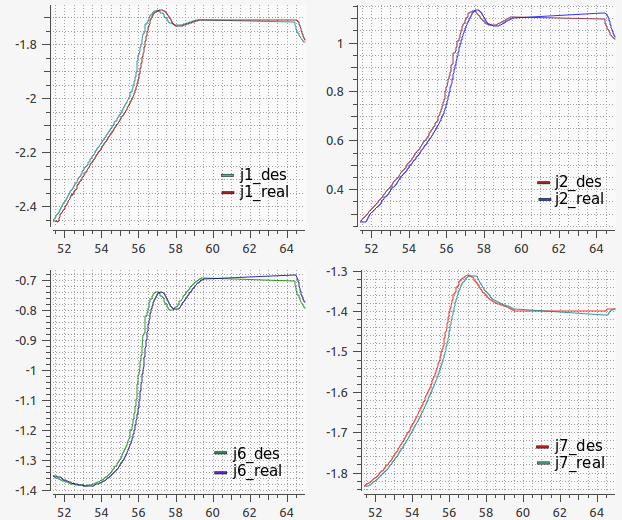
\includegraphics[width=0.7\linewidth]{pi_behavior2.png}
	\vspace{-10pt}
	\caption[Comparison: Generated and Executed trajectory]{Comparison between generated and executed trajectories. X axis - seconds, Y axis - joint values}
	\vspace{-15pt}
	\label{fig:behavior2}
\end{figure}

Figures \ref{fig:behavior} and \ref{fig:behavior2} show a comparison between the trajectory generated by the motion controller and the one executed by the robot. The first three plots if figure \ref{fig:behavior} show the behavior of the base and torso. The remaining plots show the seven joints of the arm used to grasp the object. As it can be seen, the robot follows accurately the planned trajectory.
